\section{Dimension One: A Geometric Look at the Real Line}

Although we assume the reader is familiar with the real numbers $\mathbb{R}$, it is beneficial to revisit them from a more grown-up geometric perspective to set the stage for higher dimensions. The real line is a set $\mathbb{R}$ of elements that are conventionally called numbers. However in geometry, their names and their role depends on the context. For example, when we visualize $\mathbb{R}$ as a line in space, each element corresponds to a specific location. In this context, we refer to elements of $\mathbb{R}$ as \textbf{points}.

\subsection{Translations and Vectors}

Elements of $\mathbb{R}$ have another geometric interpretation: they can represent \textbf{translations} or shifts (in this book we use the two words interchangeably). For example, the number $v \in \mathbb{R}$ can associated with the operation of shifting the origin (or any other point) by $v$ units to the right.

Formally, for any fixed number $v \in \mathbb{R}$, we can define a translation operator $T_v: \mathbb{R} \to \mathbb{R}$ by:
\[ T_v(x) = x + v \]
This operator takes a point $x$ and shifts it by $v$, obtaining the point $x+v$. When we think of elements of $\mathbb{R}$ as defining these shift operators, it is often helpful to visualize them as \textbf{arrows} rather than points, which visually correspond to the shift operation.

An arrow can be drawn starting at the origin $0$ and ending at $v$ to represent the shift $v$. However, the same shift operation can be applied to any point. Thus, we can draw an arrow starting at any point $x$ and ending at $x+v$ to represent the same shift $v$.
Formally, we can think of an arrow as a pair of points $(x, y)$, where $x$ is the \emph{tail} (or anchor) and $y$ is the \emph{head}. This arrow represents the displacement from $x$ to $y$.

\begin{figure}[h]
    \centering
    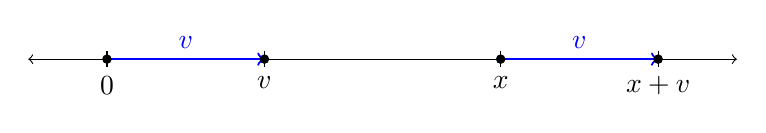
\begin{tikzpicture}
        % Number line
        \draw[<->] (-1,0) -- (8,0);
        \foreach \x in {0,2,5,7} \draw (\x,0.1) -- (\x,-0.1);
        \node[below] at (0,-0.1) {$0$};
        \node[below] at (2,-0.1) {$v$};
        \node[below] at (5,-0.1) {$x$};
        \node[below] at (7,-0.1) {$x+v$};
        
        % Vector v from origin
        \draw[->, thick, blue] (0,0) -- (2,0) node[midway, above] {$v$};
        
        % Vector v from x
        \draw[->, thick, blue] (5,0) -- (7,0) node[midway, above] {$v$};
        
        % Points
        \filldraw (0,0) circle (1.5pt);
        \filldraw (2,0) circle (1.5pt);
        \filldraw (5,0) circle (1.5pt);
        \filldraw (7,0) circle (1.5pt);
    \end{tikzpicture}
    \caption{Visualizing a vector $v$ as a translation. The blue arrows represent the same vector $v$, acting as a displacement from $0$ to $v$ and from $x$ to $x+v$. Both arrows represent the same geometric object.}
    \label{fig:vector_translation}
\end{figure}

Two arrows $(x, y)$ and $(x', y')$ are considered \textbf{equivalent} if they represent the same displacement, which means:
\[ y - x = y' - x' \]
(in which case one can define $z=y-x$, and the arrows become $(x, x+z)$ and $(x', x'+z)$ respectively)
This indeed defines an equivalence relation on the set of all arrows. An equivalence class thus contains arrows which correspond to the same displacement. Thus while each arrow in an equivalence class is a different object, they all signify the same geometric concept. We thus define a \textbf{vector} to be an equivalence class of arrows under this relation.
This vector captures the abstract notion of "magnitude and direction" (in 1D, direction is just sign) of a shift, which can be respresented by an arrow but are independent of its starting point. Note that for a vector $v$ which contains the arros $(x,y)$, $v$ is uniquely identified by the number $y-x$. We therefore sometimes say, somewhat abusing definitions, "the vector $z$" when we actually mean the equivalence class of arrows $\set{(x, x+z)}_{x\in\mathbb{R}}$. 

\subsection{Shapes and Configurations}

The construction of vectors from arrows is a specific instance of a more general pattern in geometry: defining abstract geometric objects as equivalence classes of concrete configurations.

We define a \textbf{shape} (or simply a subset) to be any subset $S \subset \mathbb{R}$. For example, the interval $[a, b] \subset \mathbb{R}$ is a shape.
Furthermore, we define a \textbf{shape configuration} (or simply a configuration) to be a tuple of shapes (which may also include single points). For example, an arrow $(x, y)$ is a configuration of two points.

For any translation $v \in \mathbb{R}$, we can translate a shape $S$ to get a new shape $S + v = \{ s + v \mid s \in S \}$. Similarly, we can translate a configuration by translating each of its components.

\subsection{Geometric Shapes and Configurations}

Intuitively, if we shift a shape like $[a, b]$ by some amount $v$, we get a new set $[a+v, b+v]$. While these are different subsets of $\mathbb{R}$, they represent the "same" geometric figure, just in different locations.

We define a \textbf{geometric shape} as an equivalence class of shapes under translation. Two shapes $A, B \subset \mathbb{R}$ determine the same geometric shape if there exists a translation $v$ such that $B = A + v$.

Similarly, we define a \textbf{geometric configuration} as an equivalence class of configurations under translation.
For instance, consider an arrow consisting of a pair of points $(x, y)$. If we shift both $x$ and $y$ by the same $z$, we get an equivalent arrow $(x+z, y+z)$. The equivalence class of this arrow configuration is precisely what we defined earlier as a \textbf{vector}. Thus, a vector is a specific type of geometric configuration.

\begin{figure}[h]
    \centering
    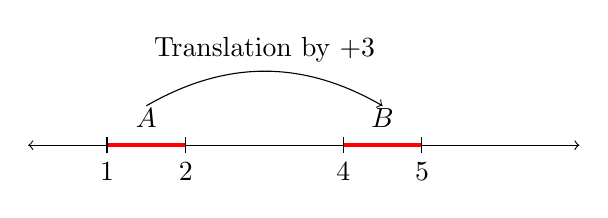
\begin{tikzpicture}
        % Number line
        \draw[<->] (0,0) -- (7,0);
        
        % Interval A [1,2]
        \draw[ultra thick, red] (1,0) -- (2,0);
        \node[above] at (1.5,0.1) {$A$};
        \draw (1,0.1) -- (1,-0.1);
        \draw (2,0.1) -- (2,-0.1);
        \node[below] at (1,-0.1) {$1$};
        \node[below] at (2,-0.1) {$2$};
        
        % Interval B [4,5] (translated by 3)
        \draw[ultra thick, red] (4,0) -- (5,0);
        \node[above] at (4.5,0.1) {$B$};
        \draw (4,0.1) -- (4,-0.1);
        \draw (5,0.1) -- (5,-0.1);
        \node[below] at (4,-0.1) {$4$};
        \node[below] at (5,-0.1) {$5$};

        % Translation arrow
        \draw[->, bend left] (1.5,0.5) to node[above] {Translation by $+3$} (4.5,0.5);
    \end{tikzpicture}
    \caption{The sets $A=[1,2]$ and $B=[4,5]$ represent the same geometric shape because one is a translation of the other.}
    \label{fig:shape_equivalence}
\end{figure}

A \textbf{geometric property} can be viewed in two equivalent ways. First, it is a property of configurations (or shapes) which is invariant under translations. For example, the property "the distance between the two points is 5" is a geometric property of a pair of points $(x, y)$, because shifting the pair does not change their distance. Equivalently, it is a property of geometric configurations (or geometric shapes). Since all configurations in an equivalence class share the same invariant properties, we can ascribe the property to the class as a whole. Thus, "length" is a property of the vector (or geometric interval) itself, independent of where it is located in space.

\paragraph{Geometric Objects.}
The term \textbf{geometric object} is a general term that encompasses geometric shapes, geometric configurations, and more. It refers to an equivalence class of any type of object for which translation is defined (this could include functions, vector fields, etc.). Whenever we have objects that can be translated, the equivalence classes under translation are the "geometric" versions of those objects.

\begin{figure}[h]
    \centering
    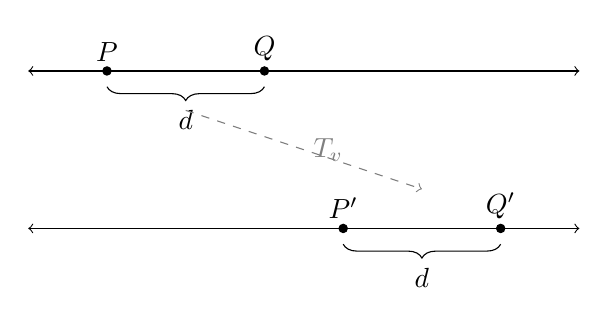
\begin{tikzpicture}
        % Configuration 1
        \draw[<->] (-1,2) -- (6,2);
        \filldraw (0,2) circle (1.5pt) node[above] {$P$};
        \filldraw (2,2) circle (1.5pt) node[above] {$Q$};
        \draw[decorate,decoration={brace,amplitude=5pt,mirror}] (0,1.8) -- (2,1.8) node[midway,below=5pt] {$d$};
        
        % Configuration 2
        \draw[<->] (-1,0) -- (6,0);
        \filldraw (3,0) circle (1.5pt) node[above] {$P'$};
        \filldraw (5,0) circle (1.5pt) node[above] {$Q'$};
        \draw[decorate,decoration={brace,amplitude=5pt,mirror}] (3,-0.2) -- (5,-0.2) node[midway,below=5pt] {$d$};
        
        % Translation arrow
        \draw[->, dashed, gray] (1,1.5) -- (4,0.5) node[midway, right] {$T_v$};
    \end{tikzpicture}
    \caption{Geometric properties, such as the distance $d$ between two points, are invariant under translation.}
    \label{fig:geometric_invariance}
\end{figure}

